\chapter{Analisi del contesto tecnologico}
\label{cap:analisi-soluzioni-esistenti}

\intro{In questa sezione vengono illustrati gli strumenti di analisi SEO più in linea con gli obiettivi del progetto, il cui studio ha fornito una base solida per la formulazione dei requisiti.}

\section{Introduzione}

\par Uno dei passi fondamentali nel processo di ottimizzazione \gls{seo} è la scelta delle parole chiave e il loro utilizzo in punti strategici delle pagine web. Esistono software in grado di automatizzare la ricerca e l'analisi delle parole chiave, contribuendo a migliorare il posizionamento e l'indicizzazione di un sito. Questi strumenti, disponibili gratuitamente o a pagamento, coprono numerosi aspetti dell'analisi SEO, tra cui:
\begin{itemize}
    \item Analisi SEO \gls{on-page} e \gls{off-page};
    \item Identificazione delle parole chiave più frequenti;
    \item Analisi della densità e della distribuzione delle parole chiave all'interno di una pagina web;
    \item Analisi dell'efficacia delle parole chiave;
    \item Ricerca delle parole chiave per cui un sito è posizionato in alto nella \gls{serp};
    \item Suggerimenti di parole chiave correlate e rilevanti;
    \item Anteprime SERP per una determinata parola chiave;
    \item Analisi dei \textit{competitor};
    \item Analisi di parametri come la \gls{keyword-difficulty} e di pratiche come il \gls{keyword-stuffing}.
\end{itemize}

\section{MozBar}

\subsection{Funzionalità}
\par \textit{MozBar} è un'estensione gratuita per Chrome che consente agli utenti di eseguire analisi SEO \gls{on-page} e \gls{off-page} senza aprire un'altra scheda del browser. Le funzionalità fornite dall'estensione includono:
\begin{itemize}
    \item \textbf{Page Authority e Domain Authority}: metriche da 1 a 100 che stimano il posizionamento di una singola pagina o di un dominio in base a un algoritmo di apprendimento automatico;
    \item \textbf{Linking Domains}: numero di domini unici che puntano a un sito;
    \item \textbf{Inbound Links}: numero di link in entrata provenienti da pagine web esterne;
    \item \textbf{Attributi generali}: tempo di caricamento, \gls{tag-canonical}, URL della cache di Google, \gls{sitemap}, \gls{hreflang}, \gls{tag-robots};
    \item \textbf{Elementi on-page}: URL, titolo, meta description, meta tag keywords, elenco degli heading, testo alternativo delle immagini;
    \item \textbf{Dati strutturati (\gls{json-ldg})}: verifica che lo schema sia formattato correttamente;
    \item \textbf{Ranking Keywords}: identifica le parole chiave per cui un sito è posizionato e fornisce informazioni sui \textit{competitor};
    \item \textbf{Ottimizzazione della pagina}: visualizza il punteggio ottenuto per una determinata parola chiave e mostra  i fattori che contribuiscono al punteggio complessivo, nonché quelli che potrebbero danneggiarlo;
    \item \textbf{Highlight links}: evidenzia tutte le tipologie di link presenti all'interno della pagina;
    \item \textbf{Highlight keywords}: questa funzionalità consente agli utenti di inserire una parola chiave e ottenere il numero di occorrenze. Inoltre, la parola chiave viene evidenziata graficamente all'interno della pagina.
\end{itemize}

\begin{figure}[H]
    \centering 
    \fbox{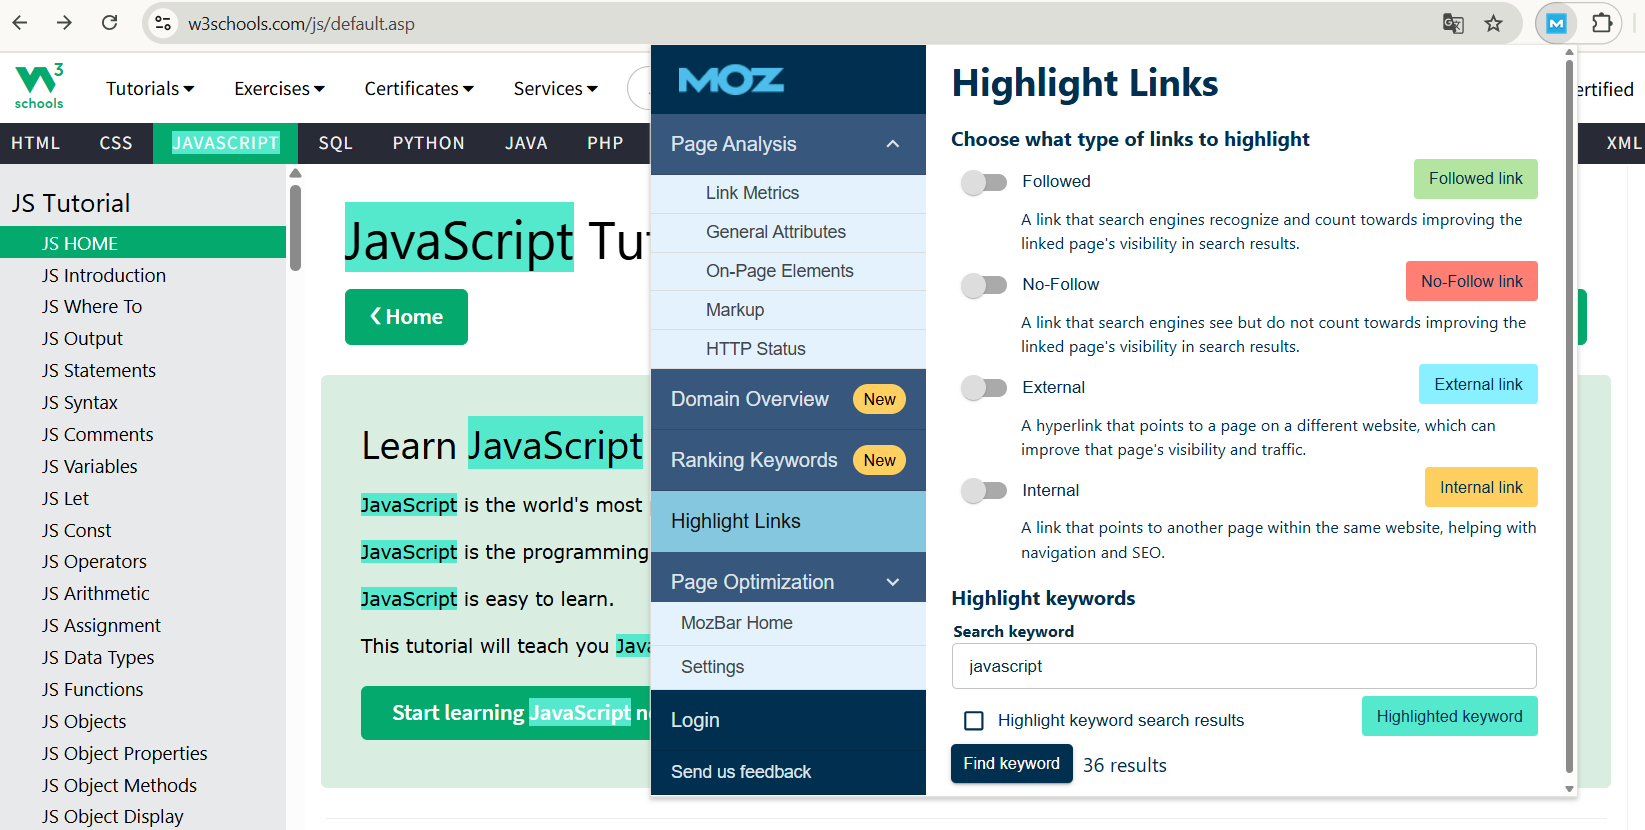
\includegraphics[width=0.9\columnwidth]{soluzioni-esistenti/MozBar/moz_bar_search_keywords.png}}
    \caption{MozBar - Analisi del sito “W3Schools”}
\end{figure}

\subsection{Vantaggi}
\par Poiché funziona su \gls{localhost}, l'estensione può essere facilmente usata durante lo sviluppo. La barra degli strumenti può essere ancorata in alto o in basso nella pagina e le metriche SEO possono essere visualizzate direttamente nei risultati di ricerca.

\subsection{Svantaggi}
\par L'estensione non è disponibile come barra laterale, ma solo come pop-up o barra degli strumenti. L'analisi delle parole chiave non include alcuni aspetti essenziali, come la densità o la distribuzione. Inoltre, il rilevamento dei tag è \gls{case-sensitive}, quindi c'è il rischio che alcuni tag non vengano individuati se si usa la lettera iniziale maiuscola. Le funzionalità Premium richiedono un abbonamento a pagamento. 

\section{Wincher}

\subsection{Funzionalità}
\par \textit{Wincher} è una piattaforma orientata alla ricerca e all'analisi delle parole chiave; in particolare, \textit{Wincher} monitora il posizionamento di un sito web, i volumi di ricerca, il traffico stimato e le anteprime \gls{serp}. La piattaforma include anche l'\textit{On-Page SEO Checker}, uno strumento di analisi \gls{on-page} per un URL e una parola chiave specifici. Il \textit{tool} fornisce suggerimenti per migliorare una pagina web in relazione alla parola chiave scelta:
\begin{itemize}
    \item \textbf{Titolo}: lunghezza del titolo, presenza e posizione della parola chiave nel titolo;
    \item \textbf{Heading}: lunghezza e numero di occorrenze del tag H1, presenza e posizione della parola chiave nel tag H1, differenza di contenuto tra il titolo e il tag H1, presenza della parola chiave nei sottotitoli;
    \item \textbf{Meta}: presenza della parola chiave nel meta tag description;
    \item \textbf{Media}: presenza della parola chiave nel testo alternativo delle immagini;
    \item \textbf{URL}: presenza della parola chiave negli URL;
    \item \textbf{Body}: la parola chiave dovrebbe essere menzionata almeno tre volte nel corpo del testo.
\end{itemize}

\begin{figure}[H]
    \centering 
    \fbox{
\includegraphics[width=0.8\columnwidth]{soluzioni-esistenti/Wincher/wincher_seo_checker.png}}
    \caption{Wincher - On-Page SEO Checker}
\end{figure}

\subsection{Vantaggi}
\par \textit{On-Page SEO Checker} fornisce un punteggio complessivo e dei suggerimenti per garantire la conformità di una pagina alle attuali linee guida SEO.

\subsection{Svantaggi}
\par Lo strumento di analisi on-page non funziona su \gls{localhost} ed è accessibile esclusivamente tramite la piattaforma di \textit{Wincher}. Nella versione gratuita, i controlli giornalieri sono limitati.

\begin{figure}[H]
    \centering 
    \fbox{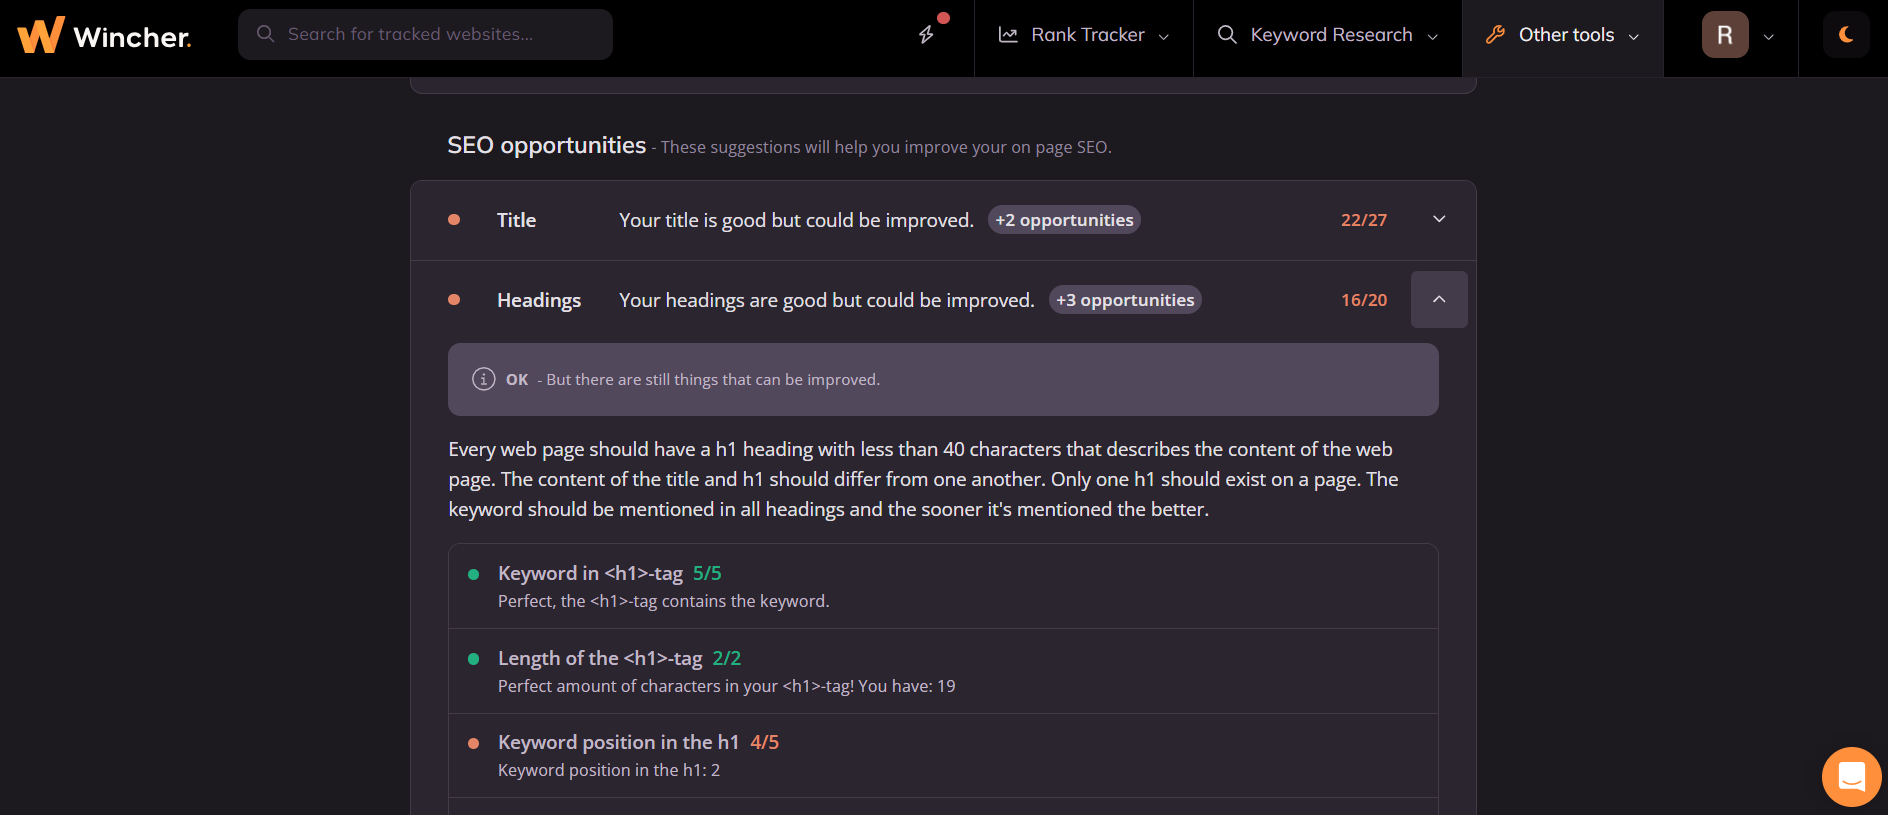
\includegraphics[width=0.8\columnwidth]{soluzioni-esistenti/Wincher/wincher_seo_checker_score.png}}
    \caption{Wincher - Analisi del sito “W3Schools”}
\end{figure}

\section{SEOquake}

\subsection{Funzionalità}
\par \textit{SEOquake} è un plugin che fornisce metriche SEO e strumenti di analisi \gls{on-page}. Le parole chiave vengono identificate tramite un algoritmo di ricerca e successivamente elencate in quattro tabelle distinte:
\begin{itemize}
    \item Keyword di 1 parola;
    \item Keyword di 2 parole;
    \item Keyword di 3 parole;
    \item Keyword di 4 parole.
\end{itemize}
\vspace{5pt}
\par\noindent Per ogni parola chiave, \textit{SEOquake} visualizza il numero di occorrenze e la densità. Inoltre, verifica se ciascuna parola chiave appare nei seguenti tag \gls{html}:
\begin{itemize}
    \item Titolo della pagina;
    \item Meta description;
    \item Meta tag keywords;
    \item Tag H1.
\end{itemize}
\vspace{5pt}
\par\noindent Tutti questi fattori contribuiscono a determinare un punteggio di importanza per ogni parola chiave. \textit{SEOquake} permette anche di filtrare le parole chiave, esportare i risultati dell'analisi in formato \gls{csv} e configurare un elenco di parole da includere o escludere.

\begin{figure}[H]
    \centering 
    \fbox{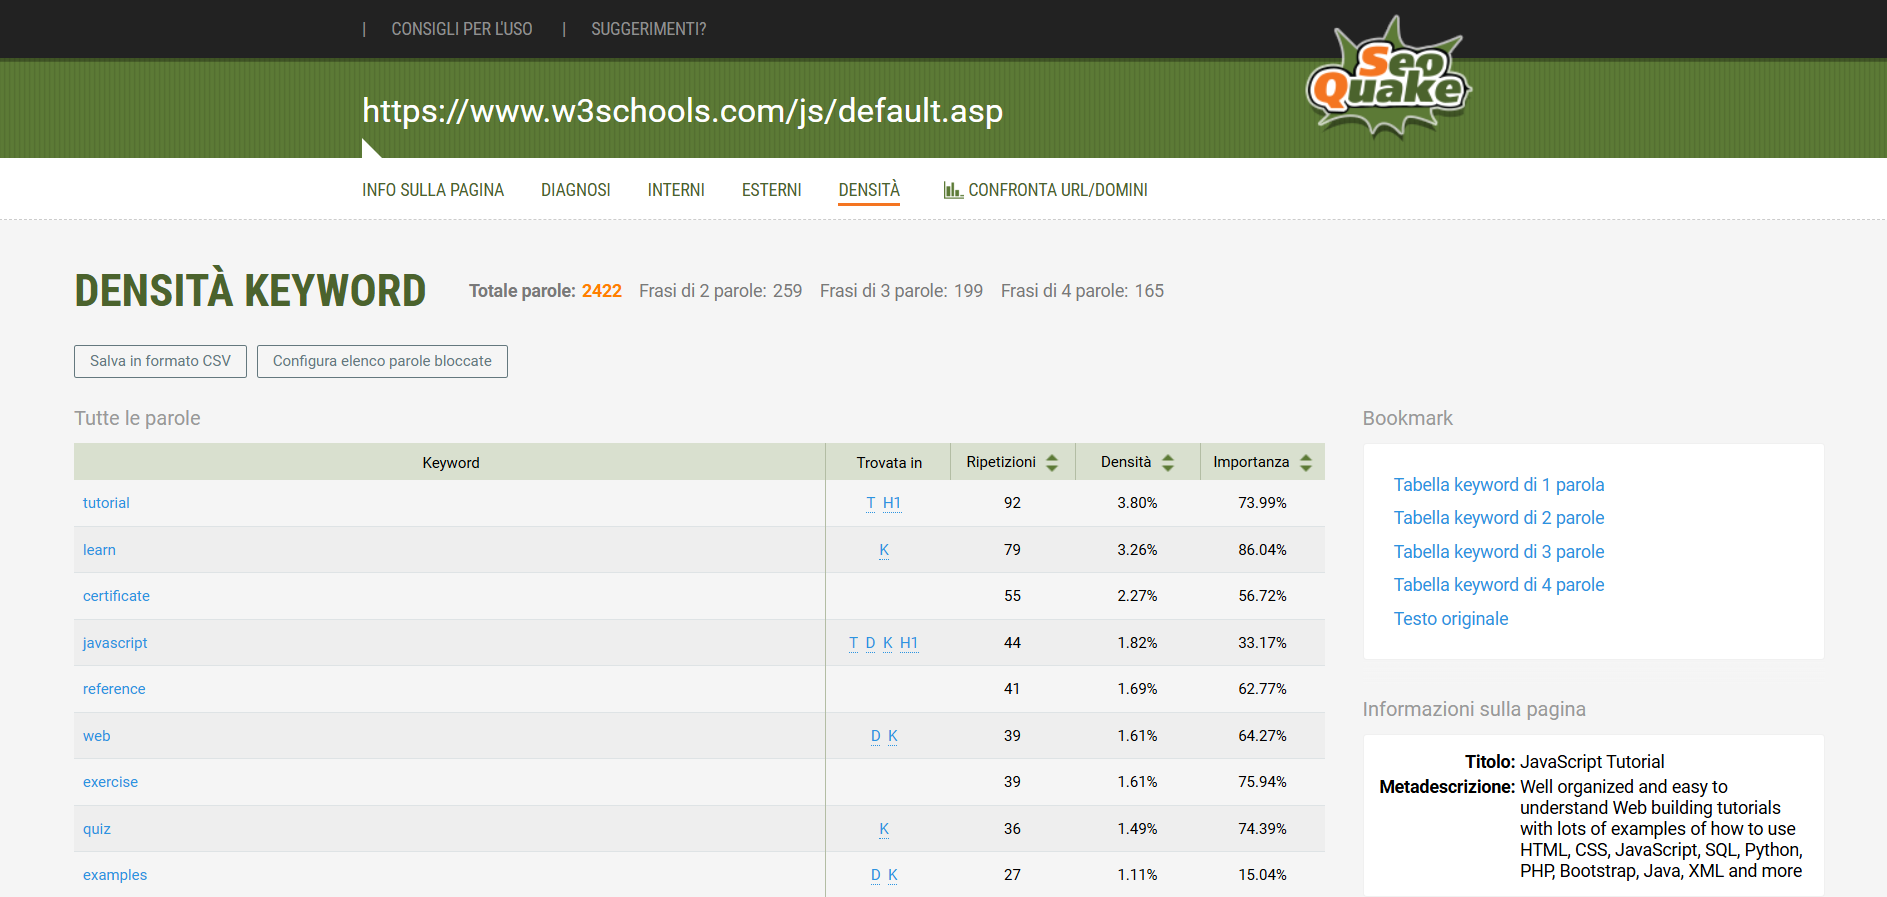
\includegraphics[width=0.9\columnwidth]{soluzioni-esistenti/SEOquake/seoquake.png}} 
    \caption{SEOquake - Analisi del sito “W3Schools”}
\end{figure}

\subsection{Vantaggi}
\par Oltre all'analisi \gls{on-page}, \textit{SEOquake} offre anche funzionalità avanzate come l'analisi dei \gls{backlink} e del traffico; il tutto è integrato in un'unica piattaforma che funziona su \gls{localhost}. L'estensione è sviluppata da \textit{Semrush} e, pertanto, include servizi propri della piattaforma.

\subsection{Svantaggi}
\par Le funzionalità di analisi SEO on-page sono accessibili solo tramite la \textit{dashboard} esterna, il che limita l'interazione diretta con la pagina corrente.

\section{SEOptimer}

\subsection{Funzionalità}
\par \textit{SEOptimer} è una piattaforma di analisi SEO e reportistica. Offre una suite completa di strumenti che coprono le seguenti funzionalità:
\begin{itemize}
    \item \textbf{Audit SEO}: fornisce un punteggio complessivo basato su fattori come SEO \gls{on-page} e \gls{off-page}, usabilità, performance e ottimizzazione per i social media;
    \item \textbf{Crawler SEO}: esegue una scansione dettagliata di una pagina web, includendo un'analisi della distribuzione delle parole chiave. Le parole chiave vengono estratte in base alla frequenza e suddivise in:
    \begin{itemize}
        \item Keyword di 1 parola;
        \item Keyword di 2 o più parole.
    \end{itemize}
    Le parole chiave dovrebbero essere distribuite correttamente tra i seguenti tag \gls{html}: 
    \begin{itemize}
        \item Titolo della pagina;
        \item Meta description;
        \item Tag di intestazione (heading).
    \end{itemize}
    \item \textbf{Monitoraggio delle parole chiave};
    \item \textbf{Ricerca di parole chiave}: analizza i \textit{competitor} e fornisce suggerimenti per nuove parole chiave;
    \item \textbf{Ricerca e monitoraggio dei \gls{backlink}}.
\end{itemize}

\begin{figure}[H]
    \centering 
    \fbox{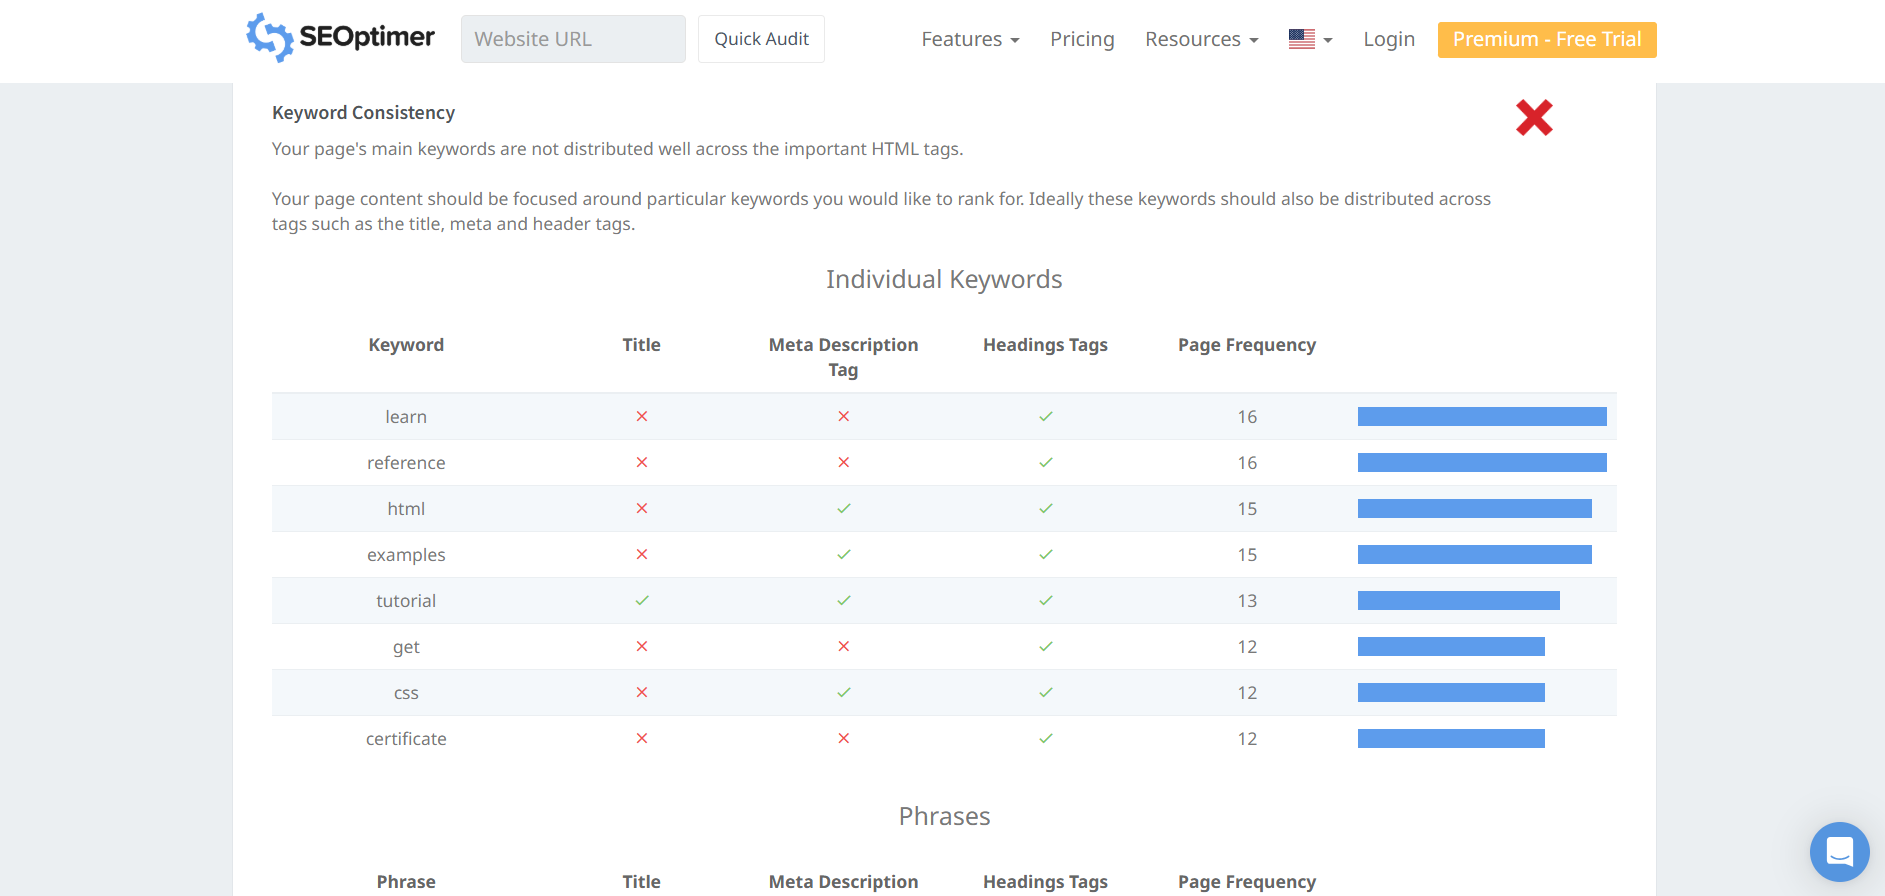
\includegraphics[width=0.9\columnwidth]{soluzioni-esistenti/SEOptimer/seoptimer.png}} 
    \caption{SEOptimer - Analisi del sito “W3Schools”}
\end{figure}

\subsection{Vantaggi}
\par \textit{SEOptimer} integra in un'unica piattaforma tutti gli strumenti necessari per un'analisi SEO approfondita ed è più economico rispetto ad altri servizi simili.

\subsection{Svantaggi}
\par \textit{SEOptimer} non funziona su \gls{localhost} e la versione gratuita consente un numero limitato di report giornalieri. Non è disponibile un'estensione per browser, pertanto l'analisi può essere eseguita soltanto tramite la piattaforma proprietaria.

\section{SEO tester online}

\subsection{Funzionalità}
\par \textit{SEO tester online} è un'estensione gratuita per Chrome sviluppata da \textit{Sitechecker}. Fornisce una panoramica generale dei dati SEO essenziali, seguita da un elenco di sezioni specifiche, tra cui:
\begin{itemize}
    \item \textbf{Contenuto}: analizza la gerarchia degli heading, la lunghezza del testo, il rapporto testo/codice \gls{html} e la densità delle keyword composte da 1, 2 o 3 parole;
    \item \textbf{Link e immagini};
    \item \textbf{\Gls{hreflang} e dati strutturati};
    \item \textbf{Velocità di caricamento};
    \item \textbf{Analisi \gls{gsc}}.
\end{itemize}

\subsection{Vantaggi}
\par L'estensione è gratuita e si integra con \gls{gsc}, offrendo un'analisi SEO completa e professionale.

\subsection{Svantaggi}
\par L'estensione non funziona su \gls{localhost} e si apre unicamente come pop-up.

\begin{figure}[H]
    \centering 
    \fbox{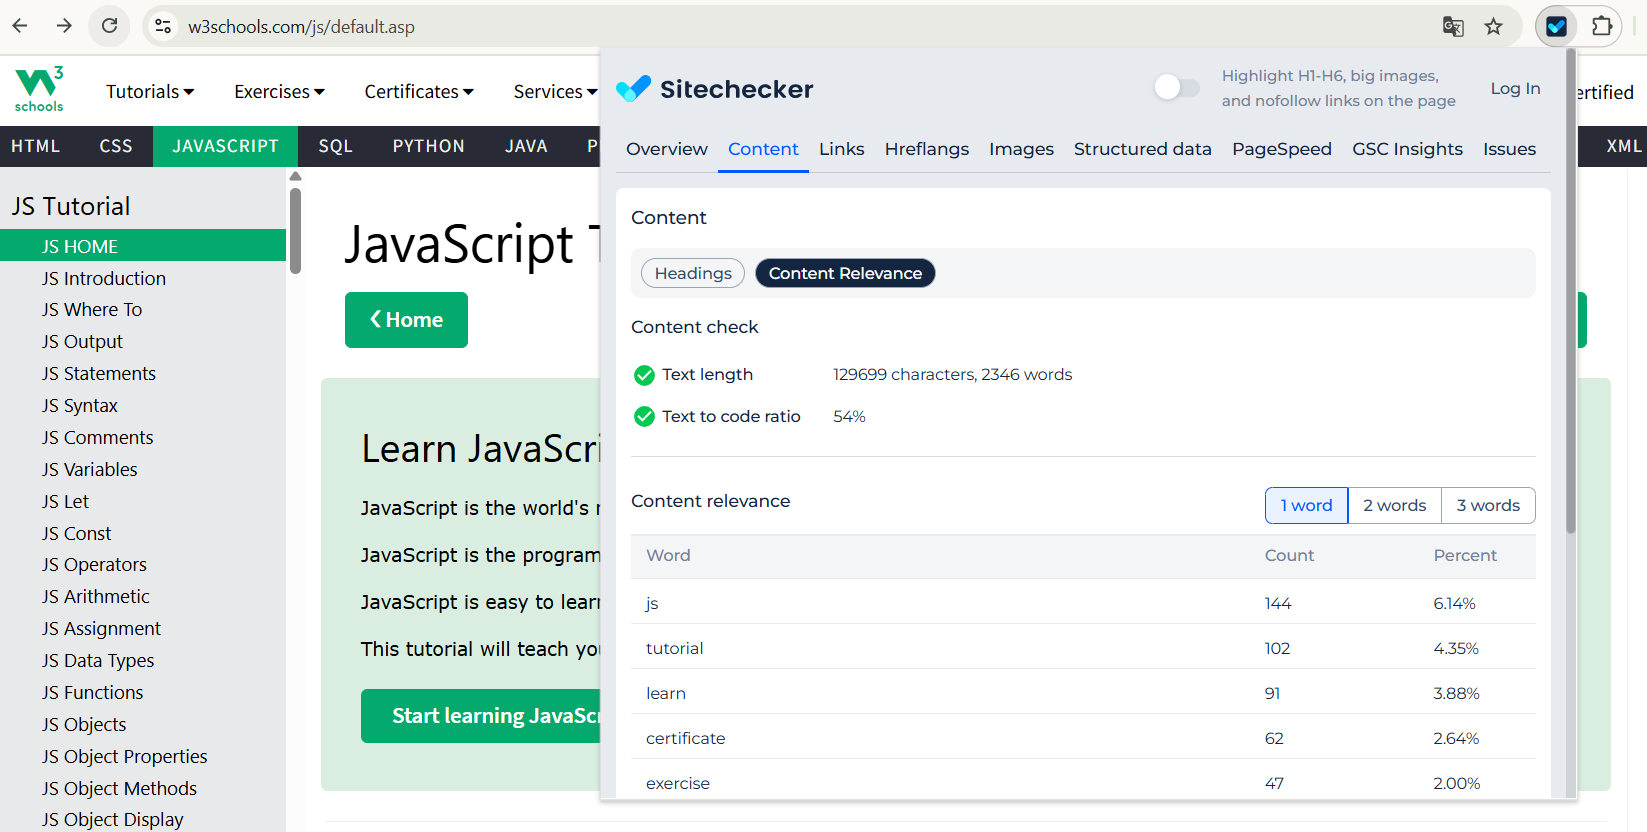
\includegraphics[width=0.9\columnwidth]{soluzioni-esistenti/SEO-Tester-Online/site_checker.png}} 
    \caption{SEO tester online - Analisi del sito “W3Schools”}
\end{figure}

\section{Semrush}

\subsection{Funzionalità}
\par \textit{Semrush} include oltre 50 strumenti di analisi SEO, il che lo rende una delle piattaforme più complete sul mercato. La \textit{dashboard} consente di visualizzare gratuitamente analisi relative al traffico, ai \gls{backlink}, alle ricerche \gls{organiche} e a quelle \gls{sponsorizzate}. In merito all’analisi delle parole chiave, \textit{Semrush} offre le seguenti funzionalità:
\begin{itemize}
    \item \textbf{Analisi SEO \gls{on-page}};
    \item \textbf{Keyword research}: suggerisce parole chiave rilevanti in base al volume di ricerca, all'intento, alla \gls{keyword-difficulty} e ad altri fattori SEO. Questa funzionalità può essere integrata con plugin di terze parti, tra cui \textit{Yoast SEO} per \gls{wordpress};
    \item \textbf{Analisi dei competitor};
    \item \textbf{Position tracking}: monitora il posizionamento nella \gls{serp} per determinate parole chiave.
\end{itemize}

\begin{figure}[H] 
    \centering 
    \fbox{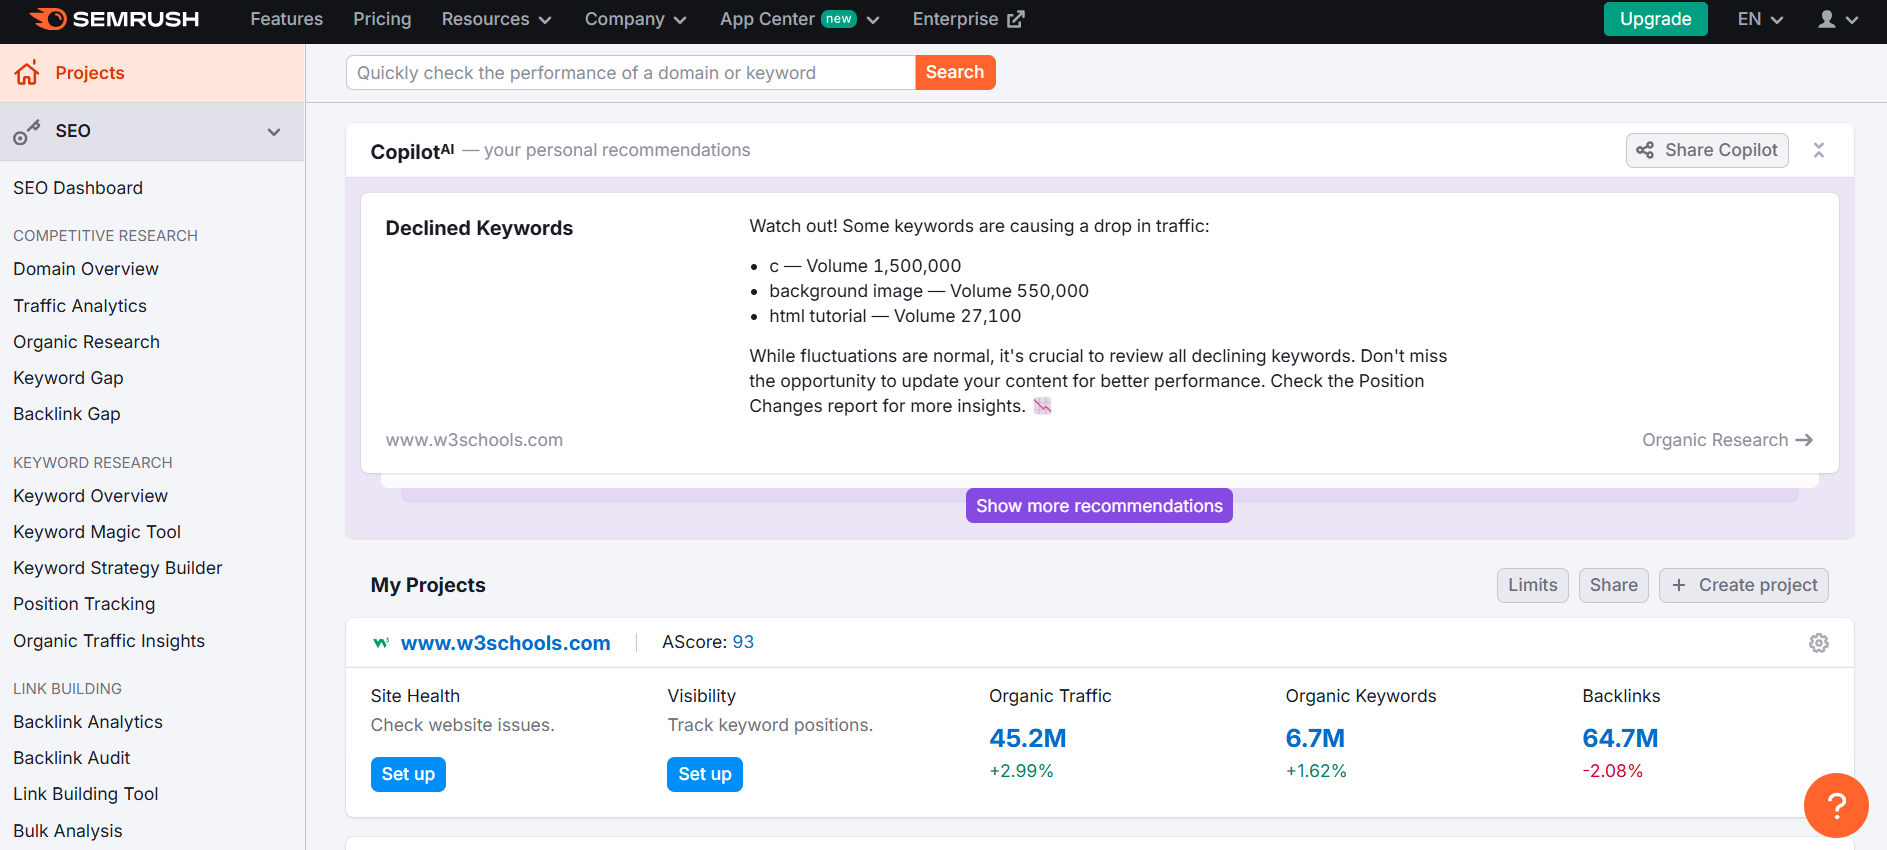
\includegraphics[width=0.8\textwidth]{soluzioni-esistenti/SEMrush/semrush.png}} 
    \caption{Semrush - SEO dashboard}
\end{figure}

\subsection{Vantaggi}
\par \textit{Semrush} può essere integrato facilmente con altri strumenti di analisi SEO.

\subsection{Svantaggi}
\par Le funzionalità avanzate sono a pagamento. Per effettuare un'analisi, è necessario interrompere la navigazione e accedere alla piattaforma web di \textit{Semrush}.

\section{Yoast SEO (plugin per CMS)}

\subsection{Funzionalità}
\par \textit{Yoast SEO} è un plugin per \gls{cms} che semplifica il processo di ottimizzazione SEO. Fornisce feedback in tempo reale per migliorare il posizionamento sui motori di ricerca. La versione del plugin per \gls{wordpress} consente di ottimizzare le parole chiave (note anche come keyphrase) attraverso un'analisi della densità, della distribuzione e di altri fattori \gls{on-page}. Con la versione a pagamento, l'utente può anche scegliere manualmente delle keyphrase correlate (argomenti collegati o parole chiave secondarie) da valutare distintamente. Inoltre, l'integrazione con \textit{Semrush} fornisce automaticamente suggerimenti di keyphrase correlate basati sui volumi di ricerca, sull'intento e sulla \gls{keyword-difficulty}. Naturalmente, i controlli sono meno restrittivi rispetto alla keyphrase principale. Per evitare di dover ripetere meccanicamente la stessa keyphrase, la versione Premium permette anche di aggiungere uno o più sinonimi, che \textit{Yoast} interpreta allo stesso modo senza penalizzare il punteggio.

\subsection{Vantaggi}
\par \textit{Yoast SEO} è disponibile in versione gratuita per \gls{wordpress}, seppur con alcune limitazioni, e può essere integrato con altri strumenti come \textit{Semrush} e \textit{Wincher}. Il plugin viene aggiornato regolarmente per rimanere allineato agli algoritmi dei motori di ricerca e alle \textit{best practice} SEO.

\subsection{Svantaggi}
\par \textit{Yoast SEO} è limitato a \gls{cms} come WordPress e \gls{shopify}. Alcune funzionalità, tra cui l'inserimento di keyphrase correlate e sinonimi, o l'integrazione con \textit{Semrush}, richiedono la sottoscrizione di un abbonamento a pagamento.

\begin{figure}[H]
    \centering 
    \fbox{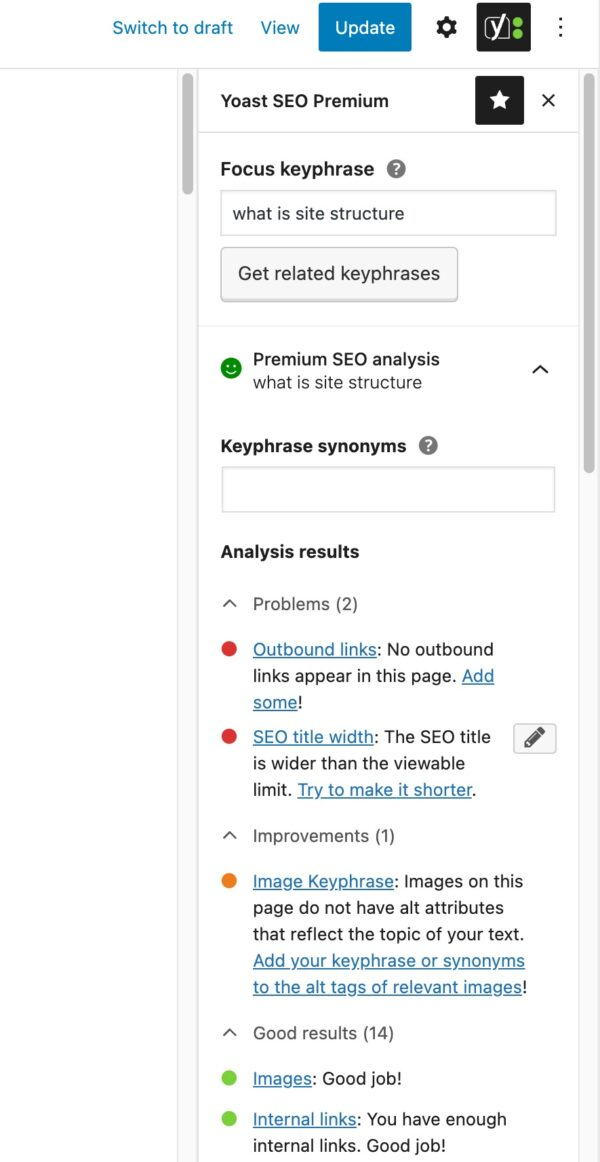
\includegraphics[width=0.4\columnwidth]{soluzioni-esistenti/Yoast-SEO/yoast_seo_premium.png}} 
    \caption{Yoast SEO Premium - Analisi SEO}
\end{figure}

\section{Keyword Density Analyzer}

\subsection{Funzionalità}
\par \textit{Keyword Density Analyzer} è uno strumento di analisi \gls{seo} fornito da \textit{Webmaster Tips}. L'analisi inizia con una panoramica generale della pagina esaminata, che include le seguenti informazioni:
\begin{itemize}
    \item URL, titolo, meta description e lingua;
    \item Dimensione della pagina non compressa;
    \item Dimensione del contenuto di testo semplice;
    \item Rapporto testo semplice/codice \gls{html};
    \item Conteggio di caratteri e parole;
    \item \textbf{Top keywords}: elenco delle parole chiave considerate più rilevanti in base a parametri interni all'applicazione.
\end{itemize}
\vspace{5pt}
\par\noindent Viene poi effettuata un'analisi del titolo e della meta description, evidenziando la frequenza e la densità di ciascuna parola contenuta in questi tag. L'analisi delle parole chiave è suddivisa in quattro sezioni:
\begin{itemize}
    \item \textbf{Meta tag keywords}: mostra la frequenza e la densità delle parole chiave specificate nel meta tag keywords;
    \item \textbf{Top Keywords by Density}: elenca le parole più frequenti, escludendo quelle comuni e troppo brevi. Oltre alla frequenza e alla densità, mostra anche il numero di occorrenze nel titolo, negli heading, nei link e nel testo alternativo delle immagini;
    \item \textbf{Top Keywords by Score}: elenca le parole in base a un punteggio calcolato internamente;
    \item \textbf{Top Phrases}: elenca le frasi con più di una occorrenza, escludendo quelle brevi e con parole comuni.
\end{itemize}

\begin{figure}[H]
    \centering 
    \fbox{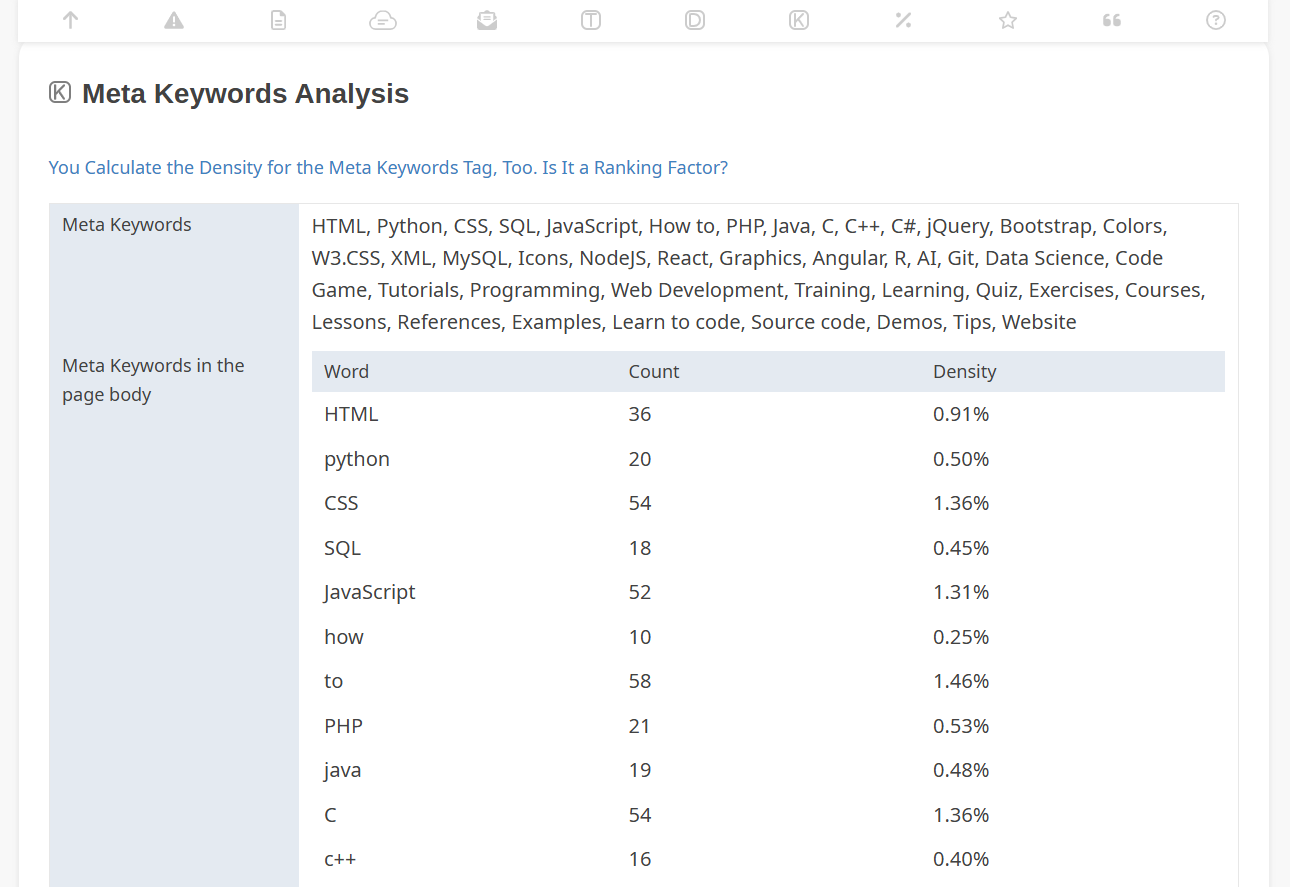
\includegraphics[width=0.8\columnwidth]{soluzioni-esistenti/Keywords-Density-Analyzer/keywords_density_analyzer.png}} 
    \caption{Keyword Density Analyzer - Analisi del sito “W3Schools”}
\end{figure}

\subsection{Vantaggi}
\par Tutte le funzionalità sono gratuite e possono essere integrate con gli altri strumenti di \textit{Webmaster Tips} per un'analisi SEO completa.

\subsection{Svantaggi}
\par L'analisi di una pagina web richiede di interrompere la navigazione e accedere alla piattaforma di \textit{Webmaster Tips}.

\begin{figure}[H]
    \centering 
    \fbox{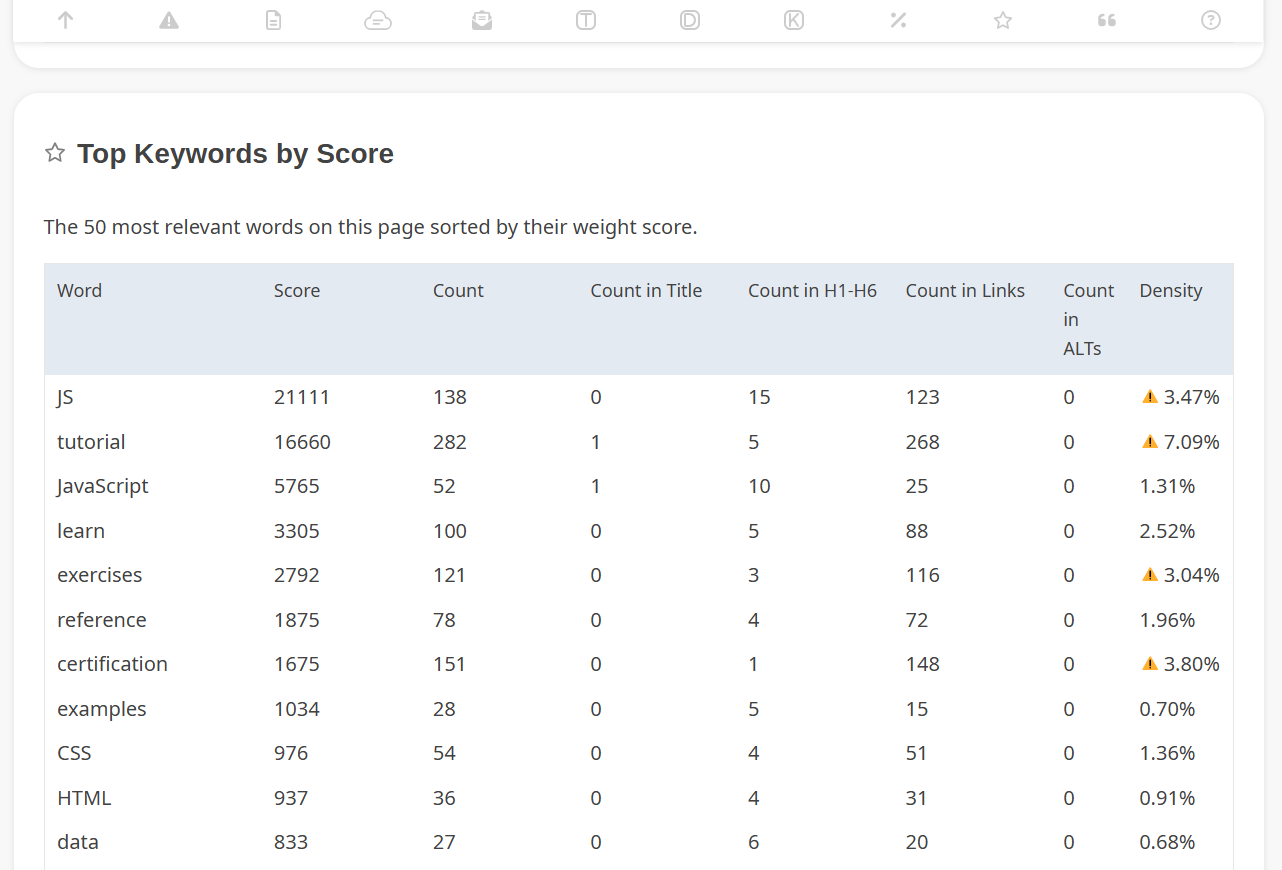
\includegraphics[width=0.8\columnwidth]{soluzioni-esistenti/Keywords-Density-Analyzer/keywords_density_analyzer_score.png}} 
    \caption{Keyword Density Analyzer - Top Keywords by Score}
\end{figure}

\section{Detailed SEO Extension}

\subsection{Funzionalità}
\par \textit{Detailed SEO Extension} è un'estensione per Google Chrome e Firefox che consente di analizzare, con un solo clic, qualsiasi sito web. L'estensione estrae e analizza i seguenti elementi:
\begin{itemize}
    \item \textbf{Overview}: Titolo, meta description, URL, \gls{tag-canonical}, \gls{tag-robots}, meta tag keywords, numero di parole e lingua;
    \item \textbf{Gerarchia degli heading} (da H1 a H6): l'estensione regola l'indentazione e la dimensione del font in base al livello, facilitando l'analisi visiva della struttura;
    \item \textbf{Link} (unici, interni o esterni, completi o incompleti);
    \item \textbf{Immagini} (complete o prive di attributi);
    \item \textbf{Schema e \gls{hreflang}};
    \item \textbf{Ottimizzazione per i social media}.
\end{itemize}
\vspace{5pt}
\par\noindent Inoltre, l'estensione genera automaticamente i link per analizzare la stessa pagina web su altre piattaforme, tra cui \textit{Ahrefs}, \textit{Majestic}, \textit{Moz}, \textit{Semrush} e \textit{SimilarWeb}.

\begin{figure}[H]
    \centering 
    \fbox{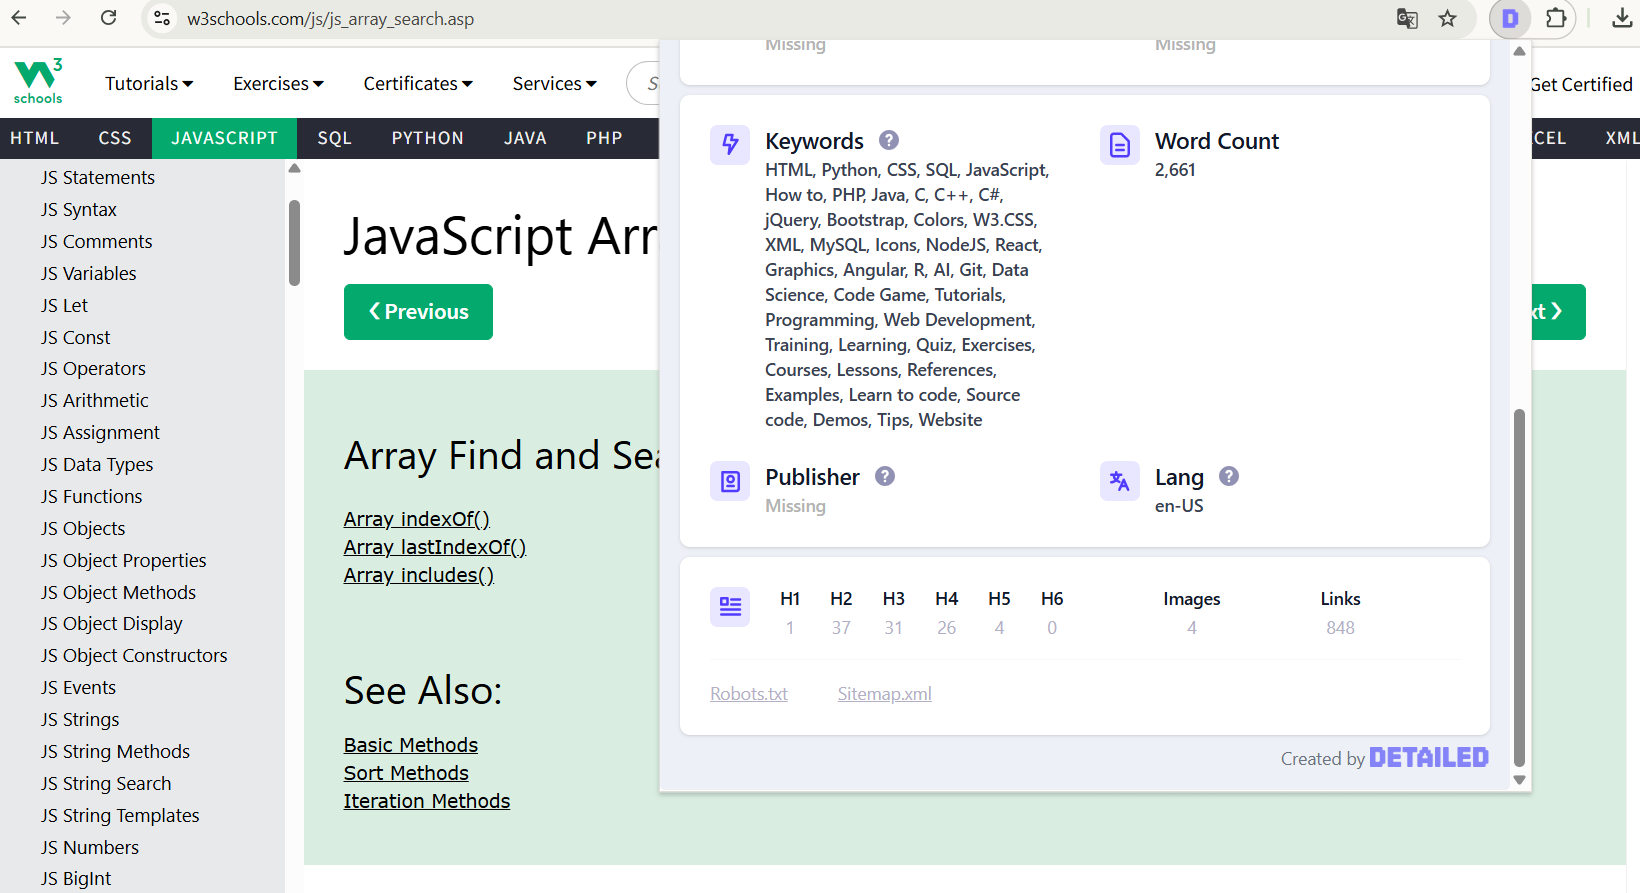
\includegraphics[width=0.8\columnwidth]{soluzioni-esistenti/Detailed-SEO-Extension/detailed_seo_analysis.png}} 
    \caption{Detailed SEO Extension - Analisi del sito “W3Schools”}
\end{figure}

\subsection{Vantaggi}
\par Essendo gratuita e compatibile con \gls{localhost}, l'estensione si presta perfettamente all'uso durante la fase di sviluppo.

\subsection{Svantaggi}
\par L'estensione si apre come pop-up, il che può rendere meno agevole l'interazione con la pagina corrente. Per quanto riguarda l'analisi delle parole chiave, lo strumento si limita a estrarre quelle presenti nel meta tag keywords.

\section{SEO Analyzer (Rank Math)}

\subsection{Funzionalità}
\par \textit{Rank Math} è un plugin per \gls{wordpress} che semplifica l'ottimizzazione SEO mediante suggerimenti basati sulle \textit{best practice}. Lo strumento \textit{SEO Analyzer} esegue un'analisi approfondita delle pagine web, generando un punteggio complessivo. Inoltre, \textit{SEO Analyzer} visualizza un elenco delle parole chiave più frequenti e verifica che siano distribuite correttamente.

\subsection{Vantaggi}
\par \textit{SEO Analyzer} è in grado di analizzare anche siti web che non sono stati realizzati con WordPress.

\subsection{Svantaggi}
\par \textit{SEO Analyzer} non funziona su \gls{localhost} ed è meno affidabile rispetto ad altri strumenti, in quanto l'analisi dei tag è \gls{case-sensitive}, il che può portare a errori come il mancato rilevamento della meta description. Inoltre, la versione Premium di \textit{Rank Math} è a pagamento.

\begin{figure}[H]
    \centering 
    \fbox{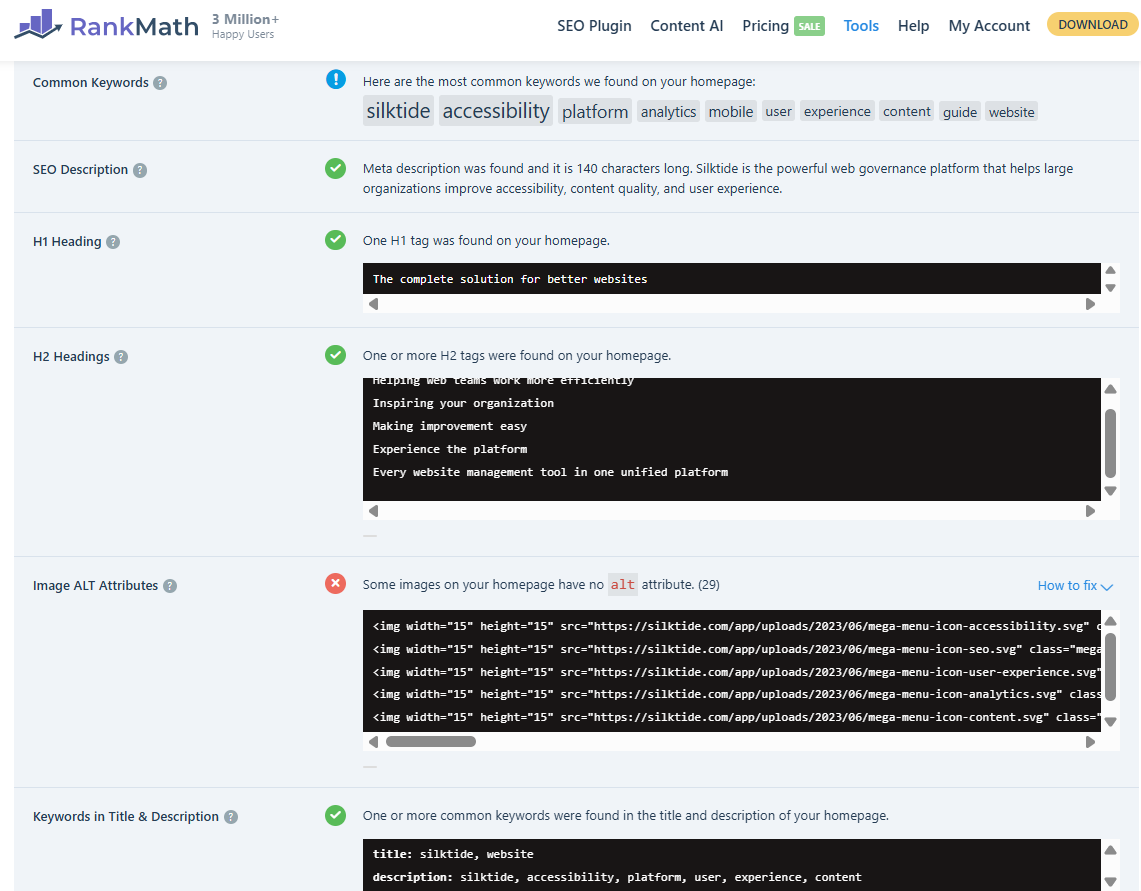
\includegraphics[width=0.7\columnwidth]{soluzioni-esistenti/RankMath/rank_math.png}} 
    \caption{Rank Math - Analisi del sito “Silktide”}
\end{figure}